\chapter{Definice pojmů}
    V této kapitole upřesňuji termíny použité ve zbytku práce. Pro nadužívané pojmy s nejasným významem vyberu jednu konkrétní definici (\textit{cloud}, \textit{continuous deployment}). Popíšu některé technologie používané porovnávanými \CI nástroji (kontejnerizace, \glstext{SAST}/\glstext{DAST}). V rámci úvodu do problematiky \CICD uvedu možnosti nahrání aplikace na web server. Uvádím také definici dostupnosti webové aplikace, na kterou se později budu odkazovat při testování \CICD nástrojů.

    \section*{Cloud}
        Na cloud se budu odkazovat v několika rovinách: jako platforma pro hostování \CI, spouštění jobů a hostování samotných aplikací, což má význam pro nasazení a tedy \CD.

        Cloudem primárně uvažuji velké organizace, které mají desítky tisíc serverů v jednom regionu \cite{pier-cloud}. Kromě hlavní trojice \glstext{AWS}, \glstext{GCP} a Azure můžeme uvažovat i DigitalOcean, IBM Cloud, Linode a celou řadu dalších globálních poskytovatelů. Kromě virtuálních serverů patří typicky do nabídky služeb managed varianty stavových aplikací jako jsou databáze, kontrolní roviny orchestrátorů, síťové disky a další. Drobnější a regionální poskytovatele cloudu, stejně tak jako on-premise cloudová řešení (OpenStack), nebudu v práci pod pojem cloud zahrnovat, protože mají jiné vlastnosti co se týče dostupnosti. Z českých hostingů nabízí „on-demand“ virtuální servery například Master Internet \cite{master-pricing}, ale jde o jiný model než velký cloud: servery se rezervují na měsíc a platí se za využitý výkon nad nějakou hranici. U jiných českých hostingových firem jsem jiné než fixní měsíční poplatky za server nenašel.

        Speciálně pro \CI je cloud vhodný cenou. Jelikož \CI má nárazové využití a to navíc ještě jenom přes pracovní hodiny, je u dedikovaných serverů výjimečně špatná utilizace. V cloudu je možné platit pouze za využité zdroje a zapínat je dynamicky. Při porovnávání \CI nástrojů budu zjišťovat, jestli a do jaké míry podporují cloud.

    \section*{Dostupnost aplikací}
        Fishman (Sun Microsystems Inc.) definuje dostupnost jako vztah mezi střední čas mezi výpadky (\glstext{MTBF}) a dobou zotavení z výpadku (\glstext{MTTR}) \cite{fishman-availability}. Dostupnost se často vulgarizuje na „počet devítek“ (99,999 \% dostupnost odpovídá pěti devítkám, což je kolem 5 minut nedostupnosti ročně). Cílem je teoretickou dostupnost maximalizovat. B.~Wilson z firmy Backblaze ale trefně dodává, že od 8. devítky jsou jakékoliv odhady čistě akademické a aplikace s větší pravděpodobností nebude fungovat kvůli ozbrojenému konfliktu \cite{backblaze-availability}.

        Aplikaci v jedné instanci na jednom fyzickém serveru lze bez výpadku provozovat. Jedním takový příkladem je server Stratus s redundantním hardwarem, který měl v jednom případě rekordní uptime 24 let \cite{thibodeau-longest-uptime}. Celý systém běží na proprietárním operačním systému, který od let 2000 nebyl aktualizovaný. Tyto servery jsou ale fyzicky na jednom místě a při přírodní pohromě nebo delším výpadku elektřiny přestanou být dostupné.

        Řešení je aplikaci provozovat distribuovaně, v několika fyzicky vzdálených datacentrech. V případě výpadku části systému se uživatelské požadavky plynule rozdělí mezi zbylé funkční systémy. Pro uživatele je tato operace transparentní a neprojeví se zhoršením dostupnosti. Provozovat a později aktualizovat distribuovanou aplikaci je relativně složité a více to popisuji v kapitole \ref{distributed-apps}. Získáme ale horizontální škálovatelnost a tím vyšší teoretickou dostupnost.

        Při testování \CICD systémů se budu zajímat o několik různých dostupností:
        \begin{itemize}
            \item Dostupnost \CICD systémů při běžném provozu;
            \item Dostupnost \CICD systémů při správě, typicky při aktualizaci na novější verzi;
            \item Podpora nasazení uživatelské aplikace v daném \CICD a dopad na dostupnost dané aplikace.
        \end{itemize}

        Žádný z velkých poskytovatelů nenabízí \glstext{SLA} pro jednu instanci (virtuální stroj). Definují pouze $99,99$~\% dostupnost na celý region (\glstext{AWS} \cite{aws-sla}, \glstext{GCP} \cite{gcp-sla}, Azure \cite{azure-sla}). V rámci regionu může bez vlivu na \glstext{SLA} vypadnout několik datacenter (\textit{availability zones}). Při porušení \glstext{SLA} vrací poskytovatelé na požádaní část kreditů. Neexistuje tak prakticky žádná garance dostupnosti a aplikace musí \glstext{HA} zajistit distribuováním mezi datacentra.

    \section*{Testování aplikací}
        Ve vhodně zvoleném \CI nástroji je možné aplikaci testovat na všech úrovních: od jednotkových (\textit{unit}) přes integrační až po funkcionální testy. Jednotkové testy v kontextu webových aplikací se uvažují maximálně o velikosti jedné stránky \cite{testing-web-apps}. V případě dostatečné dekompozice (mj.~za správného použití návrhu \glstext{MVC}) budou testované jednotky především v modelové vrstvě (byznys logice). Takové testy budou využívat pouze zkompilovanou aplikaci a případně runtime a závislosti budou simulovat atrapami (\textit{Mock objects}) \cite{mocks}. Díky tomu jsou tyto testy jednoduše spustitelné na \CI.

        Integrační testy se spouští nad moduly otestovanými jednotkově \cite{ould1986testing} a ověřují, že výsledné propojení komponent je funkční \cite{integration-tests}. Tyto testy mohou využívat externí závislosti, například databáze.

        Nejucelenějším ověřením správnosti aplikace jsou funkcionální testy (také \textit{end-to-end} testy, e2e). Při nich se aplikace spustí s externími závislostmi, simulují se uživatelské akce a monitorují se odpovědi aplikace. Ve webovém prostředí to může být volání aplikace nástrojem \code{curl}, dedikovaný testovací nástroj Selenium, nebo moderní knihovna Puppeteer pro prohlížeč Google Chrome. Co se týče nasazení na \CI jsou funkcionální testy nejkomplikovanější, protože mají řadu závislostí. Cloud může jejich nasazení zjednodušit \cite{gcp-headless}.

        %\todo{Popsat, jak lze snadno integrovat další služby jako například Messenger}\blind[1]

        Testování bezpečnosti aplikací zmíním níže v sekci o \pfxref{SAST a DAST}{sast-dast}.

    \section*{Nasazení aplikace}
        V této sekci popisuji varianty nasazení nové verze aplikace s vysokou dostupností. U porovnávaných \CICD systémů budu později zkoumat, jaké varianty nasazení podporují, případně jak obtížné je jednotlivé varianty implementovat.

        Konceptuálně je nasazení webového sofware přímočaré: vystavěný balíček aplikace se nějakým způsobem nahraje na jeden nebo více serverů a následně se spustí. Detaily se liší podle použitého prostředí. V následujícím textu jsem se zaměřil na monolitické webové aplikace, ale podobné principy fungují i pro nasazení dílčích podpůrných služeb (\textit{microservices}), které mimo \HTTP rozhraní mohou nabízet například \glstext{gRPC}, Java \glstext{RMI}, nebo jakékoliv jiné textové nebo binární protokoly.

        Komplexita nasazení drasticky narůstá, pokud vyžadujeme kontinuální dostupnost aplikace \cite{beyer2016site}. V ideálním případě by aplikace měla při nasazování změn úspěšně obsloužit všechny příchozí požadavky. Pokud neuvažujeme continuous deployment a nasazování probíhá výjimečně, může nasazení nové verze spočívat v zastavení původní verze, výpadku, a nasazení nové verze. Toto dodnes některé firmy praktikují. Například všichni tři velcí telefonní operátoři měli v roce 2018 minimálně jednu několikahodinovou odstávku webových služeb (T-Mobile \cite{tmobile-odstavka}, O2 \cite{o2-odstavka}, Vodafone 2. května 2018 a tiskovou zprávu z webu smazal). V následujícím textu se zaměřím pouze na nasazování bez výpadku dostupnosti aplikace.

        \subsection*{Hot swapping}
            Jedna varianta kontinuální dostupnosti je hot-swapping, při kterém se aplikace může upravit bez nutnosti ji vypnout. Toto je ale dostupné pouze v prostředí s \glstext{JVM} a dále například v -- na webu málo používaných -- Lisp, Erlang, Smalltalk a Elm. Při použití hot-swapping může aplikace běžet pouze v jedné instanci a nasazení nové verze aplikace tak můžeme udělat atomicky. Tím se vyhneme celé řadě problémů popsaných níže, na druhou stranu ale výrazně zhoršujeme praktickou dostupnost: server na kterém aplikace běží musí být vždy dostupný.

        \subsection*{Jednorázový přeliv provozu mezi starou a novou aplikací}
            \label{deploy-v-jedne-instanci}
            Alternativní řešení je spustit novou verzi aplikace souběžně s původní verzí a následně přesunout provoz ze staré instance na novou. V případě \glstext{PHPFPM} při zapnuté OPcache například můžeme přepsat soubory na disku a novou verzi aplikace nasadit smazáním OPcache (což se dělá pomocí rolling update \glstext{PHPFPM} workerů). Ve světě Node.js lze využít \glstext{PM2}, který abstrahuje spouštění a vypínání procesů aplikace, v Python prostředí existuje \code{pman}. Všechny tyto systémy pracují na principu load balanceru (\glstext{LB}): uživatelské požadavky chodí na jeden vedoucí proces, který si ukládá informace o běžících aplikacích na pozadí a požadavky na ně přeposílá. Tento princip je implementovatelný pro libovolnou aplikaci. Pro load balancing můžeme použít celou řadu software: PFSense, HAProxy, Nginx, Varnish, v pokročilejších infrastrukturách Envoy \textit{service mesh}, \ldots Důležité rozhodnutí při výběru \glstext{LB} je balancovaná komunikační vrstva. Layer 4 (transportní vrtva OSI modelu) \glstext{LB} přeposílají \glstext{TCP} požadavky na základě cílové \glstext{IP} adresy a portu. Je definován i Layer 3 \glstext{LB}, který se rozhoduje pouze podle cílové \glstext{IP}, ale v literatuře se zahrnuje do \glstext{L4}. Layer 7 (aplikační vrstva) \glstext{LB} přeposílají celé \HTTP požadavky. Z vyššího protokolu vyčtou víc informací, například doménu nebo jiné hlavičky, a při přeposílání požadavku tak mohou vybrat ze celé skupiny různých serverů ty, kde daná aplikace běží. Dále \glstext{L7} \glstext{LB} musí řešit \glstext{HTTPS} (\glstext{TLS} termination) a musí tak dopředu vědět, jaké domény obsluhuje. \glstext{L7} \glstext{LB} dále může reagovat i na získané \HTTP odpovědi. Díky \HTTP specifikaci idempotentních metod (\textsc{get}, \textsc{head}, \textsc{put}, \textsc{delete} \cite{http-idempotent}) lze některé požadavky zkusit znovu na jiném serveru a to bez toho, aby se původní chyba vrátila uživateli. Load balancer může u každého serveru na pozadí měřit chybovost a rozbité servery z rotace dočasně vyřadit \cite{nginx-circuit-breaker}.

            Jak \glstext{L4} tak \glstext{L7} \glstext{LB} často podporují \textit{PROXY protocol} \cite{tarreau-proxyprotocol}, který požadavek obalí vlastní hlavičkou, které je mj. původní \glstext{IP} adresa uživatele. V případě čistého \glstext{L7} load balancování lze původní \glstext{IP} vyčíst z problematické \cite{hansen-xforwardedfor} hlavičky X-Forwarded-For nebo z Forwarded rozšíření \cite{http-forwarded}. U čistého \glstext{L4} load balancování o původní \glstext{IP} příjdeme bez PROXY protokolu úplně.

            Je nutné uvažovat konzistenci napříč několika příchozími \HTTP requesty: uživatel může načíst \HTML z původní verze, ale následující \HTTP požadavek na kaskádové styly už může přijít na novou verzi aplikace.

            Tento postup můžeme aplikovat i na aplikace běžící ve víc než jedné replice. Spustíme novou verzi aplikace souběžně se startou verzí a atomicky aktualizujeme na load balanceru cíle na novou skupinu serverů. Stále ale nemusíme řešit většinu problémů, které by přinesl distribuovaný systém.

        \subsection*{Distribuovaná aplikace}
            \label{distributed-apps}
            Postup z předchozí sekce vyžaduje atomickou změnu konfigurace load balanceru. Té je těžké docílit, pokud máme více než jednu instanci load balanceru\footnote{Pokud si pod pojmem \textit{atomická změna} představíme, že po žádném požadavku zpracovávaného novou verzí konfigurace nesmí být žádný požadavek zpracováván starou konfigurací, je možných několik implementací. Jedna z nich je vyřazení všech kromě jednoho z load balancerů, což nemusí byt triviální a rychlé, pokud jsou load balancery první síťový prvek v naší infrastruktuře a nemůžeme je například snadno vyřadit z \glstext{DNS}. Další možností je změny udělat dvoukrokově: nejprve všechny kromě jednoho primárního load balanceru překonfigurovat tak, aby přeposílali všechny požadavky na tento primární load balancer. Potom lze atomicky změnit konfiguraci nejprve primárního a následně všech ostatních load balancerů.}. Další nevýhodou je, že při nasazování nové verze aplikace se po nějakou dobu zdvojnásobí nutné výpočetní zdroje (musí běžet současně $n$ starých a $n$ nových instancí aplikace). Při continuous deployment to může být velmi často, což se prodraží na nezbytné infrastruktuře. Praktický problém tohoto řešení je i samotná jednorázovost přelivu uživatelů: pokud je část aplikace rozbitá, je rozbitá pro 100 \% uživatelů.

            Vhodnější řešení je tzv. rolling update, kdy souběžně nějakou dobu provozujeme novou i starou verzi aplikace v narůstajícím poměru. Průběžně monitorujeme aplikační metriky a v případě, že se nová verze aplikace nechová podle očekávaní, můžeme nasazování pozastavit nebo úplně vrátit. Pracujeme tedy s následujícími předpoklady:
            \begin{itemize}
                \item Aplikace zároveň běží ve staré i nové verzi. Uživatelé mohou být obsluhováni novou a následně starou verzí aplikace.  Můžeme na úrovni \glstext{LB} částečně zajistit, aby uživatelé v po sobě jdoucích požadavcích byly nasměrování na stejnou verzi aplikace (\textit{session affinity, session persistence}), ale není to spolehlivé a 100 \% řešení. Používá se buď sledovací cookie nebo \glstext{IP} adresa a oboje může uživatel upravit. Kromě toho chceme umožnit tzv. \textit{rollback}, při kterém se aplikace downgraduje na předchozí verzi.
                \item Rozdělení požadavků mezi aplikace řeší několik load balancerů. Máme vysokou dostupnost, ale ztratili jsme možnost atomických úprav konfigurace.
            \end{itemize}

            Můžeme libovolně nastavit nejenom poměr aplikací, ale i jejich absolutní počty. Pokud snížíme teoretickou dostupnost, můžeme z $n$ starých verzí aplikací vypnout $n-1$ (tzn. 1 instance staré aplikace stále běží a obsluhuje 100 \% požadavků, nenastal výpadek) a následně zapnout $n-1$ nových instancí. Tím jsme minimalizovali počet nutných výpočetních zdrojů. Pokud ale máme k dispozici volné zdroje, můžeme nechat běžících $n$ původních instancí a nasadit $m$ nových. Například v \textit{Kubernetes} je tato logika abstrahována do nastavení očekávaného počtu instancí, minimálního počtu dostupných instancí a maximálního nárůstu. Při nasazování se pak postupně vypínají staré aplikace, čeká se na zapnutí nových a tak dokola, než jsou všechny instance nové aplikace. Z tohoto procesu pochází název \textit{rolling update}.

            Za těchto podmínek nemůžeme nasazovat libovolnou aplikaci. Obecně musí být aplikace zpětně nebo dopředně kompatibilní. To komplikuje databázové migrace, nebo jinou změnu formátu na sdílených (především persistentních) úložištích. Některé změny je tak nutné nasazovat dvoufázově: první nasadíme úpravu, která zajistí dopřednou kompatibilitu, a poté samotné (původně nekompatibilní) změny.


    \section*{Definice CI/CD}
        \subsection*{Continuous integration, CI}
            Nejstarší zmínka o \CI je projekt \textit{Infuse} z roku 1989 \cite{kaiser-infuse}. Jde o návrh systému testování komplexních modulárních projektů, který podle hierarchie spouští postupně jednotkové, integrační a akceptační testy.

            Fowler v článku z roku 2000 \cite{fowler-ci-original} definuje \CI jako praktiku, při které vývojáři změny začleňují do sdíleného kódu jednou denně nebo častěji. Logická funkčnost (ale ne nutně úplnost byznysových funkcí) je pak po každé změně otestována automatickými testy. Pokud testy selžou, vývojář jehož změny zapříčinily při testování problémy je informován a očekává se, že chyby opraví.

            V aktualizovaném článku z roku 2006 Fowler \cite{fowler-ci} zmiňuje užitečnost \CI serveru jako volitelnou -- ale praktickou -- podporu této praktiky. Na vhodný výběr \CI serveru se soustředí tato práce.

            Pro potřeby této práce je \CI server nástroj, který od vývojářů přijímá zdrojový kód, rozhodne jestli je akceptovatelný a vrátí booleovskou odpověď. Je vhodné -- ale ne nutné -- aby \CI server byl úzce integrovaný s nástrojem na správu repozitářů, kde po testování můžou být otestované změny přímo zařazeny do společného kódu.

        \subsection*{Continuous delivery vs Continuous deployment, CD}
            Přestože se pojmy \textit{delivery} a \textit{deployment} zkratce \CD zaměňují, mají jeden podstatný rozdíl. Při continuous delivery je kód stále udržován v nasaditelném stavu, ale samotné spouštění nasazení je manuální~\cite{cd-delivery}. Continuous deployment je rozšíření této praktiky, které nasazuje veškerý integrovaný kód automaticky~\cite{cd-versus}.

            Chad Wathington vymezuje continuous integration jako podmnožinu \CD~\cite{fowler-go}.

    \section*{Kontejnerizace}
        V \hyperref[deploy-v-jedne-instanci]{sekci \ref*{deploy-v-jedne-instanci} o nasazení aplikace v jedné instanci} zmiňuji nutnost spustit novou a starou verzi aplikace souběžně. V kontextu \HTTP aplikací to může být problém, protože stará verze aplikace blokuje systémový port a nová verze aplikace se kvůli tomu nemůže na stejném portu zapnout. Jedno z řešení je nastavovat aplikační port při startu, což ale dále komplikuje nastavení load balanceru. Snadněji a hlavně bez úpravy aplikace lze v moderních operačních systémech využít kontejnerizace. Za použití primitiv z \glstext{LXC} (\textit{Linux Containers}) nebo abstrakce jako jsou Docker, rkt nebo containerd můžeme aplikaci spustit v izolovaném prostředí a pod známým portem. Pro jiné než Linuxové systémy existují různé alternativy, například Solaris má vlastní \textit{Solaris Containers}.

        Kontejnerizace má celou řadu dalších výhod. Díky tomu, že v obrazu (\textit{Docker image}) jsou kromě samotné aplikace i všechny nezbytné systémové závislosti; typicky knihovny vyžadované k dynamickému linkování, nebo runtime pro interpretované jazyky (například \glstext{JRE}). Mezi další výhody patří zabudované automatické cachovaní kompilace vrstev Docker obrazu a snadná distribuce obrazů.

        \label{sec:dind}
        Jeden z problémů, který při stavění kontejnerů budu muset řešit, je zanořování Dockeru. První vrstva je prostředí, ve kterém se spouští jednotlivé \CI joby. Kontejnerizace na této úrovni přináší lepší kontrolu závislostí a izolaci, ale není nutná. To je vesměs nezávislé na tom, jaké aplikace se budou na \CI stavět. Druhá vrstva, ve které se Docker může využívat, je stavění Docker obrazů v rámci konkrétního \CI jobu. Přístup k Dockeru na této úrovni nelze ničím nahradit. Jedna možnost zanořování se označuje \textit{Docker in Docker} (\glstext{DinD}, \pfxref{diagram}{fig:dind-ci}), při které všechny kontejnery stále sdílí jedno linuxové jádro, ale vnitřní kontejner je řízen Docker démonem spuštěným uvnitř vnějšího kontejneru.

        \begin{iffigure}
            \centering
            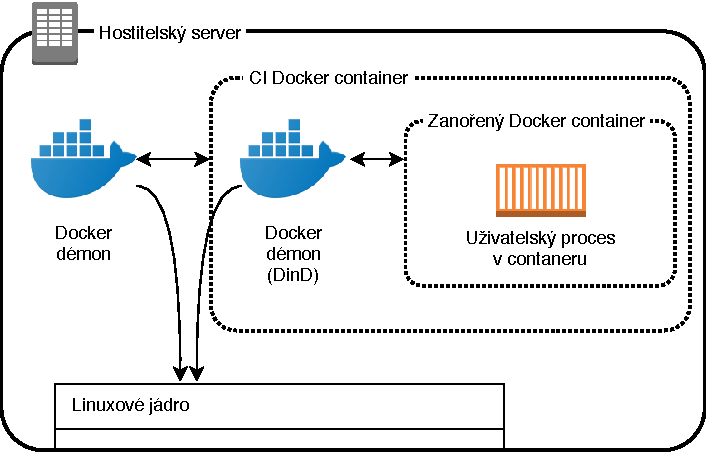
\includegraphics[width=\textwidth]{media/dind-ci.pdf}
            \caption{Diagram použití Dockeru v Dockeru.}
            \label{fig:dind-ci}
        \end{iffigure}

        Speciálně pro testování je kontejnerizace nejlepší možné řešení. Testy je často potřeba spouštět na několika různých místech, minimálně na lokálních zařízeních všech vývojářů a na \CI. S kontejnery odpadá nutnost instalovat celé testovací prostředí, které se navíc ještě víc blíží tomu produkčnímu. Díky tomu, že vývojáři a \CI spouští testy (skoro) úplně stejně, odpadají z velké části problémy kde testy lokálně prochází, ale na \CI ne. Kontejnery také zjednodušují začleňování nových vývojářů, kteří místo instalace všech závislostí a komponent mohou rovnou upravovat a spustit aplikaci.

        Nasazování aplikace se kontejnerizací také usnadňuje. Na \CI se nějakým deterministickým způsobem vytvoří Docker obraz a nahraje se do registru. Webové servery se pak informují o nové verzi, obraz stáhnou a spustí novou verzi aplikace. Odpadají tak některé problémy s atomicitou nasazení, s postupným nahrazováním a případně mazáním souborů. Další výhodou je, že vývojáři mohou lokálně spustit produkční verzi aplikace -- například pro odlazení chyby.

    \section*{Bezpečnost}
        V následující kapitole budu porovnávat různé \CI nástroje a jedním z kritérií na které se zaměřím je bezpečnost. V rámci jedné organizace není žádoucí, aby všichni uživatelé viděli všechny ostatní testované projekty. Příklad z praxe jsou zaměstnanci bez podepsaného \glstext{NDA} nebo ve zkušební době.

        Samostatná kategorie bezpečnosti \CI je izolace spuštěným jobů. Rozlišují se následující úrovně:
        \begin{itemize}
            \item Žádná izolace. Všechny joby se navzájem ovliňují. Globální závislosti jako jsou runtime, databáze atp.~jsou předinstalované.
            \item Kontejnerizace. Všechny joby sdílí společný hardware, ale každý job běží ve vlastním kontejneru a není nijak ovlivněn ostatními joby, ani se navzájem nevidí.
            \item Virtuální stroje (\glstext{VM}). Joby se spouští nad virtualizovaným hardware a odlišným jádrem. Není omezeno na Linux.
            \item Serverová/fyzická izolace. Každý job běží na jiném fyzickém serveru. Toto je prakticky velmi těžko dosažitelné, ale do jisté míry se lze tomuto ideálu přiblížit v cloudu, kde jsou stovky fyzických serverů. Přes to že hardware je sdílený, je pro potenciálního útočníka prakticky nemožné zajistit si kolokaci v krátkém čase co job běží.
        \end{itemize}

        Kontejnerizace je praktická, ale nedostačující izolace pro sdílená \CI. Pokud se útočníkovi podaří z kontejneru utéct, má plnou kontrolu nad hostitelským systémem a i všemi joby. Přesně taková zranitelnost byla nalezena v únoru 2019 v nástroji runc, který využívají Docker, Containerd, CRI-O a další a také orchestrační technologie nad nimi postavené: Kubernetes, Docker Swarm, … (CVE-2019-5736~\cite{CVE-2019-5736}). V rámci jedné organizace ale může být kontejnerizace dobrý kompromis mezi rychlostí, využitím zdrojů a bezpečností.

        Dále u \CI budu zmiňovat možnosti testování bezpečnosti aplikace. To lze rozdělit na dvě kategorie: statická analýza (\glstext{SAST}) a dynamická analýza (\glstext{DAST}). Rozdíly obou přístupů popisují následující odstavce.

        \label{sast-dast}
        \glstext{SAST} je statická analýza aplikačního kódu bez jeho spuštění~\cite{sast}. Příkladem ve světě jazyka C je volání \code{printf(argv[1])}, které by mělo být nahrazeno za \code{printf("\%s", argv[1])}. Kvalitní kompilátory mají nějakou formu \glstext{SAST} zabudovanou. \glstext{LLVM} pro ukázkový \code{printf} vygeneruje \textit{warning: format string is not a string literal (potentially insecure)}. Pro většinu programovacích jazyků a frameworků existuje nějaký externí statický analyzér (pro \glstext{PHP} phpstan, pro bash shellcheck, pro Dockerfile hadolint, …).

        \glstext{DAST} je testování bezpečnosti aplikace při jejím běhu \cite{dast}. Často skenují různé body ze seznamu \glstext{OWASP} Top 10. Přestože žádný scanner nemůže najít všechny bezpečnostní chyby~\cite{netsparker-scanner}, jsou tyto nástroje užitečné.

    \section*{Verzování závilostí}
        Uchovávání knihoven třetích stran (tzv.~\textit{vendoring}) je kontroverzní: někdo rozvážně nepreferuje ani jednu variantu~\cite{copes-commit-npm}, ale oba přístupy mají svoje problémy. Toto rozhodnutí částečně souvisí s \CI, protože potřebujeme buď stahovat externí závislosti, nebo kontrolovat jejich aktuálnost.

        %(například JavaScriptové \glstext{NPM} \todo{abbr} moduly)

        Nevýhodou přidání závislostí do repozitáře je zvětšení repozitáře, což má negativní dopad na rychlost mnoha operací a podle druhu \CICD pipeline přímý dopad na rychlost nasazování. Další problém je znepřehlednění rozdílů mezi jednotlivými verzemi v systému a při nevhodném použití verzovacího systému to může velmi komplikovat merge operace~\cite{should-i-vendor}.

        Výhody verzování externích závislostí jsou mnohé~\cite{andrawos2017cloud}. Při buildu \CICD pipeline nemusí stahovat zdroje mimo samostatného repozitáře, což zvyšuje dostupnost při výpadku cizí služby (klasické závislosti jsou GitHub, JavaScript balíčky \glstext{NPM}, pro Javu Maven central repository). Aplikace se vždy buildí s předem známými a neměnnými verzemi závislostí, takže i při nezamknutí verze balíčku se při vydání breaking change nic nerozbije (v \glstext{PHP} composer.json, v \glstext{NPM} package.json, pro Java Maven pom.xml). Tento problém lze alternativně také řešit verzováním lockfile pro daný balíčkovací systém (composer.lock, package.lock/yarn.lock, Maven lockfile nemá); problém ale může stále nastat, pokud na cizím úložišti někdo otagovanou verzi balíčku přepíše. To se může stát buď omylem nebo třeba s nekalými úmysly a spoléhání na cizí úložiště při buildu tak lze považovat za bezpečnostní riziko. Při verzování závilostí mohou všechny zdrojové soubory podléhat kontrole. Dále verzování řeší projekty smazané \cite{williams-left-pad}. Další výhodou je snadná úprava kódu závislostí bez nutnosti publikovat změny třetím stranám a čekat na integraci~\cite{rusnavcko2014fedora}.
